%%%%%%%%%%%%%%%%%%%%%%%%%%%%%%%%%%%%%%%%%%%%%%%%%%%%%%%%%%%%%%%%%%%%%%%%%%%%%%%%
%2345678901234567890123456789012345678901234567890123456789012345678901234567890
%        1         2         3         4         5         6         7         8

%\documentclass[journal,transmag]{IEEEtran}% Comment this line out if you need a4paper

\documentclass[10pt, conference]{ieeeconf}      % Use this line for a4 paper


\IEEEoverridecommandlockouts                              % This command is only needed if 
                                                          % you want to use the \thanks command

%\overrideIEEEmargins                                      % Needed to meet printer requirements.

% See the \addtolength command later in the file to balance the column lengths
% on the last page of the document

% The following packages can be found on http:\\www.ctan.org
%\usepackage{graphics} % for pdf, bitmapped graphics files
%\usepackage{epsfig} % for postscript graphics files
%\usepackage{mathptmx} % assumes new font selection scheme installed
%\usepackage{times} % assumes new font selection scheme installed
%\usepackage{amsmath} % assumes amsmath package installed
%\usepackage{amssymb}  % assumes amsmath package installed

\newtheorem{theorem}{Theorem}[section]
\newtheorem{lemma}[theorem]{Lemma}
\newtheorem{proposition}[theorem]{Proposition}
\newtheorem{corollary}[theorem]{Corollary}
\usepackage[ruled,vlined]{algorithm2e}
\usepackage{url}
\newenvironment{definition}[1][Definition]{\begin{trivlist}
\item[\hskip \labelsep {\bfseries #1}]}{\end{trivlist}}

\newcommand{\qed}{\nobreak \ifvmode \relax \else
      \ifdim\lastskip<1.5em \hskip-\lastskip
      \hskip1.5em plus0em minus0.5em \fi \nobreak
      \vrule height0.75em width0.5em depth0.25em\fi}

\def\lc{\left\lfloor}   
\def\rc{\right\rfloor}

\usepackage{amsmath,amssymb}

\usepackage{tabularx}
\usepackage{tikz,hyperref,graphicx,units}
\usepackage{subfigure}
\usepackage{benktools}
\usepackage{bbm}
\renewcommand{\baselinestretch}{.5}

\usepackage{caption}
\usepackage{epstopdf}
\renewcommand{\captionfont}{\footnotesize}
\usepackage{sidecap,wrapfig}
\usepackage[ruled,vlined]{algorithm2e}
\DeclareMathOperator*{\argmin}{arg\,min}
\DeclareMathOperator*{\argmax}{arg\,max}
\newcommand{\abs}[1]{\lvert#1\rvert} 
\newcommand{\norm}[1]{\lVert#1\rVert}
%\newcommand{\suchthat}{\mid}
\newcommand{\suchthat}{\ \big|\ }
\newcommand{\ba}{\mathbf{a}}
\newcommand{\bb}{\mathbf{b}}
\newcommand{\bc}{\mathbf{c}}
\newcommand{\bd}{\mathbf{d}}
\newcommand{\bg}{\mathbf{g}}
\newcommand{\bj}{\mathbf{j}}
\newcommand{\bn}{\mathbf{n}}
\newcommand{\bp}{\mathbf{p}}
\newcommand{\bw}{\mathbf{w}}
\newcommand{\bt}{\mathbf{t}}
\newcommand{\bu}{\mathbf{u}}
\newcommand{\by}{\mathbf{y}}
\newcommand{\bx}{\mathbf{x}}
\newcommand{\bz}{\mathbf{z}}
\newcommand{\bbf}{\mathbf{f}}
\newcommand{\bzero}{\mathbf{0}}
\newcommand{\bG}{\mathbf{G}}
\newcommand{\bA}{\mathbf{A}}
\newcommand{\bW}{\mathbf{W}}
\newcommand{\bX}{\mathbf{X}}
\newcommand{\mX}{\mathcal{X}}
\newcommand{\mD}{\mathcal{D}}
\newcommand{\mG}{\mathcal{G}}
\newcommand{\mN}{\mathcal{N}}
\newcommand{\mW}{\mathcal{W}}
\newcommand{\mF}{\mathcal{F}}
\newcommand{\bZ}{\mathbf{Z}}
\newcommand{\bbZ}{\mathbb{Z}}
\newcommand{\mR}{\mathcal{R}}


\newcommand{\bfc}{W}
\newcommand{\Qinf}{Q_{\infty}}
\newcommand{\st}[1]{_\text{#1}}
\newcommand{\rres}{r\st{res}}
\newcommand{\pos}[1]{(#1)^+}
\newcommand{\depth}{\operatorname{depth}}
\newcommand{\dist}{\operatorname{dist}}
\newcommand{\convhull}{\operatorname{ConvexHull}}
\newcommand{\minksum}{\operatorname{MinkowskiSum}}

\newcommand{\specialcell}[2][c]{ \begin{tabular}[#1]{@{}c@{}}#2\end{tabular}}
\newcommand{\acro}{SHIV}
\newcommand{\ns}{HC }
\newcommand{\nc}{RC }
\newcommand\independent{\protect\mathpalette{\protect\independenT}{\perp}}
\def\independenT#1#2{\mathrel{\rlap{$#1#2$}\mkern2mu{#1#2}}}

\newcolumntype{L}[1]{>{\RaggedRight\hspace{0pt}}p{#1}}
\newcolumntype{R}[1]{>{\RaggedLeft\hspace{0pt}}p{#1}}

%\newtheorem{lemma}{Lemma}[section]
%\newtheorem{theorem}{Theorem}[section]
\newtheorem{defn}{Definition}[section]

\newboolean{include-notes}
\setboolean{include-notes}{true}
\newcommand{\adnote}[1]{\ifthenelse{ \boolean{include-notes}}%
 {\textcolor{blue}{\textbf{#1}}}{}}
 
 \newcommand{\sknote}[1]{\ifthenelse{ \boolean{include-notes}}%
 {\textcolor{blue}{\textbf{SK: #1}}}{}}
 
  \newcommand{\mlnote}[1]{\ifthenelse{ \boolean{include-notes}}%
 {\textcolor{purple}{\textbf{ML: #1}}}{}}
 
 \newcommand{\jmnote}[1]{\ifthenelse{ \boolean{include-notes}}%
 {\textcolor{orange}{\textbf{JM: #1}}}{}}

\renewcommand{\baselinestretch}{.95}
\usepackage{times}
\usepackage{microtype}
%\title{Iterative Imitation Learning with Reduced Human Supervision [v11]}
%\title{SHIV:  Reducing Human Supervision for Robot adaptive Learning [v11]}

\title{Comparing Human-Centric and Robot-Centric \\
Sampling for Robot Deep Learning from Demonstrations}



\author{Michael Laskey, Caleb Chuck, Jonathan Lee, Jeffrey Mahler,\\ Sanjay Krishnan, Kevin Jamieson, Anca Dragan, Ken Goldberg}
\begin{document}


\maketitle
\thispagestyle{empty}
\pagestyle{empty}


%%%%%%%%%%%%%%%%%%%%%%%%%%%%%%%%%%%%%%%%%%%%%%%%%%%%%%%%%%%%%%%%%%%%%%%%%%%%%%%%




%%%%%%%%%%%%%%%%%%%%%%%%%%%%%%%%%%%%%%%%%%%%%%%%%%%%%%%%%%%%%%%%%%%%%%%%%%%%%%%%

\begin{abstract}
Motivated by recent advances in Deep Learning for robot control, this paper considers two learning algorithms in terms of how they acquire demonstrations. ``Human-Centric" (HC) sampling is the standard supervised learning algorithm, where a human supervisor demonstrates the task by teleoperating the robot to provide trajectories consisting of state-control pairs.  ``Robot-Centric" (RC) sampling is an increasingly popular alternative used in algorithms such as DAgger, where a human supervisor observes the robot executing a learned policy and provides corrective control labels for each state visited.  RC sampling can be tedious for human supervisors and prone to mislabeling.  RC sampling can also reduce sample efficiency because it repeatedly visits areas of the state space that are avoided once the task is learned. Although RC sampling can be superior to HC sampling for standard learning models such as linear SVMs, HC sampling performs equally well or better with emerging classes of highly-expressive learning models such as deep learning and hyper-parametric decision trees.  We compare HC and RC using a simulated grid world and a physical robot singulation task where the input is a binary image of a connected set of objects on a planar worksurface and the policy generates a motion of the gripper to separate one object from the rest.  In HC, humans demonstrate the task by tele-operating a four-axis robot and in RC, humans provide corrective labels to trajectories generated by the robot after an initial training phase.  We find that for linear SVMs, RC is significantly more efficient than HC but that with deep models this advantage disappears.  We also find that with RC, the corrective control labels provided by humans are highly inconsistent (uncorrelated with their own previous labels) and that deep models trained with HC can perform significantly better than with RC.  We then prove that there exists a class of examples where in the limit, HC is guaranteed to converge to an optimal policy while RC may fail to converge. These results suggest the somewhat surprising result that HC sampling may be preferable for highly-expressive learning models like deep learning.
 \end{abstract}



\section{Introduction} 
For many sequential robot tasks such as driving, walking, and manipulation where the task dynamics and reward function are not precisely known, one promising approach is Learning from Demonstrations (LfD), where a robot learns to perform a task using examples provided by a human supervisor \cite{pomerleau1989alvinn,abbeel2008apprenticeship,argall2009survey,ross2010reduction,laskeyshiv}. It is well-known that depending on the complexity of the task and the complexity of the learning model, LfD can require many demonstrations, i.e. have low sample efficiency. Learning algorithms such as DAgger have been shown to increase sample efficiency for linear models. An emerging class of highly non-linear learning models such as Deep Learning Networks and decision trees with thousands of parameters have also been shown to increase sample efficiency.  Understanding the relative benefits of the learning algorithm vs the learning model motivates a study of DAgger-like methods in the context of Deep Learning from Demonstrations (DLfD).

We consider two classes of learning algorithms that differ in how they acquire demonstrations. ``Human-Centric" (HC) sampling is the standard supervised learning algorithm, where a human supervisor demonstrates the task by tele-operating the robot to provide trajectories consisting of state-action pairs.  ``Robot-Centric" (RC) sampling is an increasingly popular alternative used in algorithms such as DAgger, where a human supervisor observes the robot executing a learned policy and retro-actively provides corrective control labels for each state visited ~\cite{ross2010efficient,ross2010reduction,laskeyrobot,laskeyshiv,he2012imitation}.  

RC sampling can be tedious for human supervisors and prone to mislabeling.  RC sampling can also reduce sample efficiency because it repeatedly visits areas of the state space that are avoided once the task is learned. Although RC sampling can be superior to HC sampling for standard learning models such as linear SVMs, HC sampling may perform equally well or better with emerging classes of highly-expressive learning models such as deep learning and hyper-parametric decision trees.


\begin{figure}
\center
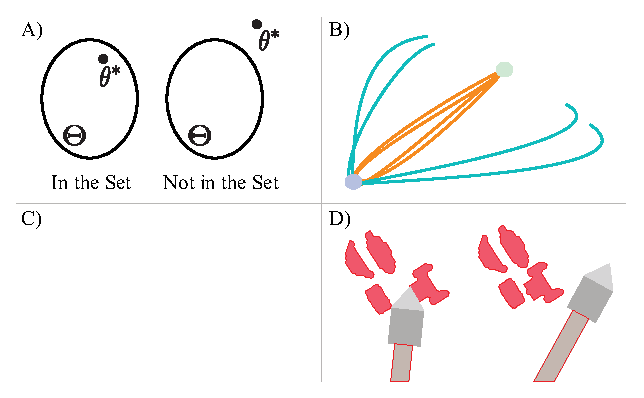
\includegraphics[width=0.5\textwidth]{f_figs/teaser.eps}
\caption{
    \footnotesize
HC and RC trajectories used to learn a robot singulation task: top view of 4 objects on a planar worksurface.  Left: In HC, 10 trajectories where a human demonstrates the task by tele-operating a four-axis robot to separate one object from a connected set of objects. Right: In RC, after initial training, 10 trajectories of the highly-suboptimal robot policy are executed and a  human provides corrective control labels for each.  Note that the latter trajectories spend considerable time in areas of the workspace that will not be useful after the task is learned.}
\vspace*{-20pt}2
\label{fig:teaser}
\end{figure}

Although RC can be more efficient for linear learning models, it requires the human supervisor to estimate the best control for counter-intuitive states which can be tedious and prone to error.  RC sampling also visits states that may not be useful after the task is learned. For example, consider the task of singulating an object from a set of objects on a table (Fig. \ref{fig:teaser}). Standard demonstrations involve moving forward and from side to side to push obstacles out of the way. However, when the robot during learning makes large errors (Fig. \ref{fig:teaser}(right)), counter-intuitive recovery motions will be required.  This can delay or prevent convergence.
 
This paper explores the value of this extra overhead for emerging classes of highly-expressive models such as deep learning and decision trees. These learners can more quickly and accurately learn the supervisor policy compared to less expressive learners such as linear models~\cite{vapnik1992principles}.

We first perform experiments with a simulated grid world. By varying the expressiveness of the robot's policy, we find on 100 randomly generated grid world environments that the performance gap between the two methods diminishes as the expressiveness is increased. Next, using a point mass control example, we find that RC sampling can fail to converge in cases when HC converges.

We then compare the two in physical experiments. We performed a pilot study with 10 students at UC Berkeley under Human Subjects Protocol Approval X.
In this experiment, each student used RC and HC sampling to train a Zymark robot to singulate an object. We observed a statistically significant gap in the average performance of the policies trained by the two approaches. For $60$  trajectories, RC had a success rate of $40\%$ compared with  $60\%$, for HC. We studied the data to identify possible reasons for this difference and found that with RC, control labels provided by the students were highly inconsistent.

%, suggesting that RC is more difficult for human supervisors. We also found that the RC policy had a higher test loss than the HC policy, suggesting that examples collected with RC sampling are more difficult to learn.
%In our post analysis, we examine how well people could match their controls in retroactive feedback compared to teleoperation. Furthermore, we analyze a held out test set's surrogate loss to explain how well the policy learned can generalize to unseen data. A higher test loss can indicate harder to learn examples were in the dataset. 

We also provide two theoretical contributions consistent with these results. First, we prove by construction that there exist a class of examples where HC converges but RC may not.  We also contribute a new analysis for the error accumulation in HC sampling for  squared Euclidean loss and normally distributed stochastic policies, which demonstrates a tighter bound than shown in prior work~\cite{ross2010efficient}. 

%move to Conclusion: Overall, our results suggest that for highly expressive deep learners, it may be more advantageous to get demonstrations using HC sampling than to ask the human supervisor for retroactive feedback along the robot's current policy.


\section{Related Work}
Below we summarize related work in HC and RC LfD and their theoretical insights. 

\noindent \textbf {\ns}  Pormeleau et al. used \ns to train a neural network to drive a car on the highway via demonstrations provided by a supervisor. To reduce the number of examples needed to perform a task, they synthetically generated images of the road and following labels~\cite{pomerleau1989alvinn}.  A similar approach was used by Dilmann et al. to teach a robot to insert perform peg-in-hole using a neural network controller~\cite{dillmann1995acquisition}. Schulman et al. used HC LfD for rope tying using kernelized interpolation as the policy class~\cite{schulman2016learning}.  A comprehensive list of HC LfD techniques can be found here~\cite{argall2009survey}. 

Ross et al. examined \ns  derived that the error in the worst case from this approach can go quadratic in the time horizon, $T$~\cite{ross2010efficient}. The intuition behind this analysis is that if the distribution induced by the robot's policy is different than the supervisor's, the robot could incur the maximum error. Expressive policies can manage constant $T$ factors by achieving very low training error. We also show that a rate of $T\sqrt{T}$ is achievable for stochastic policies. 

\noindent \textbf{\nc}
\nc has been used in numerous robotic examples, including flying a quadcopter through a forest where the state space is image data taken from an onboard sensor~\cite{ross2013learning}. Other successful examples have been teaching a robotic wheelchair to navigate to target positions~\cite{kim2013maximum}, teaching a robot to follow verbal instructions to navigate across an office building {duvallet2013imitation} and teaching a robot to grasp in clutter~\cite{laskeyrobot}.

Algorithmic extensions to \nc have also been recently made, such as forcing the supervisor to provide controls that are easier for the robot to learn from~\cite{he2012imitation}.  Kim et al. proposed only to query the supervisor in states that the robot is uncertain~\cite{kim2013maximum} . Laskey et al. extended this approach to high-dimensional states~\cite{laskeyshiv}. Laskey et al. examined a hierarchy of supervisors (ranked by quality)  to reduce the burden on an expert demonstrator~\cite{laskeyrobot}. Zhang and Cho trained a classifier to detect when \nc would encounter dangerous states during policy execution~\cite{zhang2016query}.

Ross et al.~\cite{ross2010reduction} analyze RC sampling as online optimization. The propose DAgger, an RC sampling algorithm, and show that the error for the robot's policy is linear in $T$ for strongly convex losses (i.e.  regularized linear or kernelized regression). 
However, the error also depends on the expected loss on the data collected during RC, which may be high due to observing complex recovery behaviors. We analyze this effect and show how it can prevent RC from converging to the supervisor's policy in Section \ref{sec:PS}

\textbf{LfD Interfaces:}
Standard techniques for providing demonstrations to a robot are teleoperation, kinesthetic and waypoint specification~\cite{akgun2012keyframe,akgun2012novel,argall2009survey}. Kinesthetic teaching is defined as moving the robot body via a human exerting force on the robot itself. Teleoperation uses an interface such as a joystick or video game controller to control the position of the robot end effector. Waypoint specification, or Keyframes, has a human select positions in the space that the robot needs to visit. These methods are forms of HC sampling because the human guides the robot through the task. 

Previous work has studied these HC sampling techniqes~\cite{akgun2012keyframe,akgun2012novel} relative to each other. However, in our analysis look specifically at teleoperation and compare it to RC's form of retroactive feedback. 

\section{Problem Statement and Background}\label{sec:PS}
The objective of LfD is to learn a policy that matches that of the supervisor on a specified task that demonstrations are collected on.

\noindent\textbf{Modeling Choices and Assumptions:}  We model the system dynamics as Markovian, stochastic, and stationary. Stationary dynamics occur when, given a state and a control, the probability of the next state does not change over time. 

We model the initial state as sampled from a distribution over the state space.
We assume a known state space and set of controls. We also assume access to a robot or simulator, such that we  can sample from the state sequences induced by a sequence of controls.
Lastly, we assume access to a supervisor who can, given a state, provide a control signal label.
We additionally assume the supervisor can be noisy. 

\noindent\textbf{Policies and State Densities.}
Following conventions from control theory, we denote by $\mathcal{X}$ the set consisting of observable states for a robot task, such as images from a camera, or robot joint angles and object poses in the environment.
We furthermore consider a set $\mathcal{U}$ of allowable control inputs for the robot, which can be discrete or
continuous. We model dynamics as Markovian, such that the probability of state $\mathbf{x_{t+1}}\in
\mathcal{X}$ can be determined from the previous state $\mathbf{x}_t\in\mathcal{X}$ and control input $\mathbf{u}_t\in
\mathcal{U}$: 
$$p(\bx_{t+1}|\bu_{t},\bx_{t}, \ldots, \bu_{0}, \bx_{0})=p(\bx_{t+1}|\bu_{t}, \bx_t)$$
We assume a probability density over initial states $p(\bx_0)$.
The environment of a task is thus defined as a specific instance of a control and state space, initial state distribution, and dynamics. 


%We denote the probability density over the initial state also by $p:\mathcal{X}\to \mathbb{R}$. 

Given a time horizon $T\in \mathbb{N}$, a trajectory $\tau$ is a finite sequence of $T+1$ pairs of states visited and corresponding
control inputs at these states, $\tau = ((\mathbf{x}_0,\mathbf{u}_0), ...., (\mathbf{x}_T,\mathbf{u}_T))$, where $\bx_t\in \mathcal{X}$
and $\bu_t\in \mathcal{U}$ for $t\in \{0, \ldots, T\}$.


A policy is a measurable function $\pi: \mathcal{X} \to \mathcal{U}$ from states to control inputs. 
We consider policies $\pi_{\theta}:\mathcal{X}\to \mathcal{U}$ parametrized by some $\theta\in \Theta$. Under our assumptions, any such policy $\pi_{\theta}$ induces a probability density over the set of  trajectories of length $T+1$: $$p(\tau | \theta)=
p(\bx_0)\prod_{i=0}^{T-1}p(\bx_{t+1}|\bu_t,\bx_t)p(\bu_t|\bx_t,\theta)$$


The term $p(\bu_t|\bx_t,\theta)$ indicates stochasticity in the applied control, which can occur due to noise in robot execution~\cite{mahler2014learning}.
While we do not assume knowledge of the distributions corresponding to: $p(\bx_{t+1}|\bx_t,\bu_t)$, $p(\bx_0)$ or $p(\bx_t|
\theta)$, we assume that we have a stochastic real robot or a simulator such that for any state
$\bx_t$ and control $\bu_t$, we can observe a sample $\bx_{t+1}$ from the density $p(\bx_{t+1}|\bu_t,\bx_t)$. 
Therefore, when `rolling out' trajectories under a policy
$\pi_{\theta}$, we utilize the robot or a simulator to sample the resulting stochastic trajectories rather than
estimating $p(\bx|\theta)$ itself.


\noindent\textbf{Objective.} The objective of policy learning is to find a policy that minimizes some known reward function $R(\tau) = \sum^T_{t=1} r(\bx_t,\bu_t)$ of a trajectory $\tau$. The reward $r:\mathcal{X}\times \mathcal{U}\to \mathbb{R}$ is typically user defined and task specific. 
For example in the task of grasping, the reward can be a binary measure of success.

In our problem, we do not have access to the reward function itself. Instead, we only have access to 
a supervisor, $\pi_{\theta^*}$, where $\theta^*$ may not be contained in $\Theta$. A supervisor is chosen that can achieve a desired level of performance on the task.

We measure the difference between controls using a surrogate loss $l : \mathcal{U} \times \mathcal{U} \rightarrow \mathbb{R}$~\cite{ross2010reduction,ross2010efficient}.
The surrogate loss can either be an indicator function as in classification or a continuous measure on the sufficient statistics of $p(\bu|\bx,\theta)$.
We measure total loss along a trajectory with respect to the supervisor's policy $\pi_{\theta^*}$ by $J(\theta, \tau) = \sum^T_{t=1} l(\pi_{\theta}(\bx_{t}),\pi_{\theta^*}(\bx_{t}))$.

\noindent \textbf{LfD with \ns Sampling:} In \ns the supervisor provides the robot a set of $N$ demonstration trajectories $\lbrace \tau^1,...,\tau^N \rbrace$ sampled from $p(\tau | \theta^*)$.
This induces a training data set $\mathcal{D}$ of all state-control input pairs from the demonstrated trajectories.
The goal is to find a parameter $\theta$ generates the sample demonstrations from the supervisor's policy.
\ns frames this  question as maximizing the conditional likelihood of the sample demonstrations conditioned on a given parameter $\theta$. 

$$\underset{\theta}{\mbox{max}} \prod^N_{n=1} p(\bx_{0,n}) \prod^T_{t=1} p(\bx_{t+1,n}|\bx_{t,n},\bu_{t,n})p(\bu_{t,n}|\bx_{t,n},\theta)$$

It is common to optimize the conditional log-likelihood, which maintains the same solution but breaks up the product terms into sums. 

\begin{equation}\label{eq:m_likeli_obj}
\underset{\theta}{\mbox{max}} \sum^N_{n=1}\sum^T_{t=1}\mbox{log }p(\bu_{t,n}|\bx_{t,n},\theta)
\end{equation}
\noindent We note that the dynamics and initial state distributions are dropped in this objective because they are conditionally independent of $\theta$, once the controls are observed. 

Traditionally maximizing the probability of a given control from the supervisor has been viewed as minimization the surrogate loss $l$~\cite{ross2010reduction,ross2010efficient}.
This rewrites the objective as follows: 

\begin{equation}\label{eq:main_obj}
\theta^N = \underset{\theta}{\mbox{argmin }} \sum \limits_{i=1}^N J(\theta, \tau_i).
\end{equation}

\noindent \textbf{LfD with \nc Sampling.}
Due to sample approximation and learning error, one potential issue with \nc sampling is that $\theta^N$ differs from $\theta^*$.
Therefore it is possible that new states will be visited under $\theta^N$ that would never have been visited under $\theta^*$.
To account for this, prior work has proposed iterative solutions~\cite{ross2010reduction} that attempt to solve this problem by aggregating data on the state distribution induced by the current robot's policy.

Instead of  minimizing the surrogate loss in Eq. \ref{eq:main_obj},  LfD with RC sampling~\cite{ross2010reduction,laskeyshiv,he2012imitation} attempts to approximate the state distribution the final policy will converge to and minimize the surrogate loss on this distribution.
A popular RC sampling algorithm is DAgger~\cite{ross2010reduction}, which iterates two steps:

\subsubsection{Step 1}
The first step of any iteration $k$ is to compute a $\theta_k$ that minimizes surrogate loss on the current dataset $\mathcal{D}_k=\{(x_i,u_i)|i\in\{1,\ldots,N\}\}$ of demonstrated state-control pairs (initially just the set $\mathcal{D}$ of initial trajectory demonstrations):

 \vspace{-1ex}
\begin{align}\label{eq:super_objj}
\theta_{k} = \underset{\theta}{\argmin} \: \sum_{i=1}^{N} \sum_{t=1}^T  l(\pi_{\theta}(\bx_{i,t}),\bu_{i,t}).
\end{align}

\noindent Note that equal weight is given to each example regardless of how likely they are under the current policy.
 

 \subsubsection{Step 2}
The second step at iteration $k$, DAgger rolls out the current policy, $\pi_{\theta_{k}}$, to sample states that are likely under $p(\tau|\theta_{k})$.  For every state visited, DAgger requests the supervisor to provide the appropriate control/label. Formally, for a given sampled trajectory  $\tau = (\bx_0,\bu_0,...,\bx_T,\bu_T )$, the supervisor provides labels $\tilde{\bu}_t$, where $\tilde{\bu}_t \sim \tilde{\pi}(\bx_t) + \epsilon$, where $\epsilon$ is a  zero mean noise term, for $t\in \{0, \ldots, T\}$.
The states and labeled controls are then aggregated into the next data set of demonstrations $\mathcal{D}_{k+1}$:
$$D_{k+1}=\mathcal{D}_k \cup \{(\bx_t,\tilde{\bu_t})|t\in\{0,\ldots,T\}\} $$

\noindent Steps 1 and 2 are repeated for $K$ iterations or until the robot has achieved sufficient performance on the
task\footnote{In the original DAgger the policy rollout was stochastically mixed with the supervisor, thus with
    probability $\beta$ it would either take the supervisor's action or the robots. The use of this stochastically mix
    policy was for theoretical analysis and in practice, it was recommended to set $\beta = 0$ (i.e. RC only) to avoid biasing the
sampling~\cite{NIPS2014_5421,ross2010reduction}}.


 


\section{Empirical Analysis}

\begin{figure*}
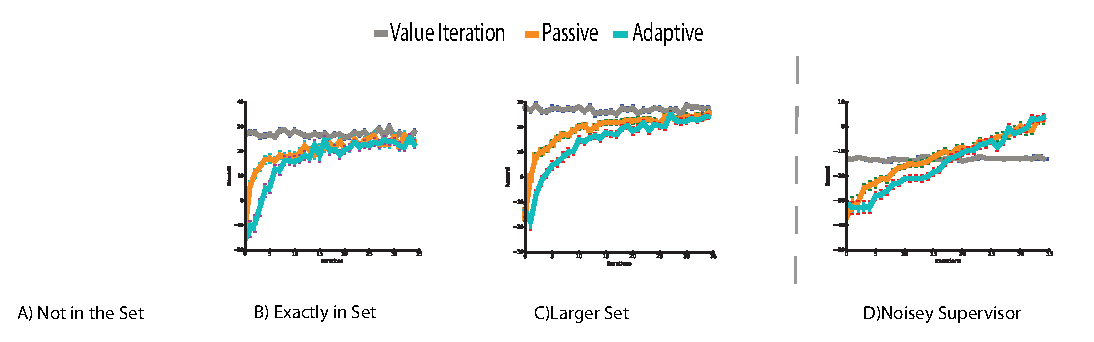
\includegraphics{f_figs/var_grid.eps}
\caption{
    \footnotesize
We compare RC and HC sampling for low- and high-expressiveness policy classes (a and b respectively) over 100 randomly generated 2D gridworld environments, as a function of the amount of data provided to them. RC outperforms in the low-expressive condition, but the performance gap is negligible in the high-expressive condition, when the policy class contains the expected supervisor policy. We also examine the case of noisy supervisor labels (c), in which both techniques take more data to converge, but again perform similarly. 
}
\vspace*{-20pt}
\label{fig:var}
\end{figure*}

We first provide an empirical comparison of HC and RC. 
We start with experiments in a Grid World environment, which enables us to vary the robot's policy class over a large number of randomly generated environments. Then we examine a linear dynamical system, which we use to exemplify a potential limitation in the ability of RC to match the supervisor's performance when it must learn complex recovery actions.
Finally, we compare HC and RC on a real task. We perform a pilot study with 10 participants, who try to teach a robot how to singulate, or separate an object from clutter. We used DAgger as the example of an RC method in these experiments. 

\subsection{Effect of Function Class}\label{sec:gdw}
In this experiment, we hypothesize that on random problems with a perfect simulated supervisor, the performance gap of RC diminishes as the robot's policy becomes more expressive. 

In Grid World, we have a robot that is trying to reach a goal state, at which it receives $+10$ reward. The robot receives $-10$ reward if it touches a penalty state. The robot also receives a $-0.02$ penalty for every blank state. The robot must learn to be robust to the noise in the dynamics, reach the goal state and then stay there.
The robot has a state space of $(x,y)$ coordinates and a set of actions consisting of $\lbrace$Left, Right, Forward, Backward, Stay$\rbrace$ state. The grid size for the environment is $30 \times 30$. $20\%$ of randomly drawn states are marked as a penalty, while only one is a goal state. For the transition dynamics, $p(\bx_{t+1}|\bx_{t},\bu_t)$, the robot goes to an adjacent state different from the one desired uniformly at random with probability $0.2$. The time horizon for the policy is $T=30$. 

We use Value Iteration to compute an optimal supervisor. In all settings we provided RC with one initial demonstration from HC sampling before iteratively rolling out its policy. This initial demonstration set from HC sampling is common in methods like DAgger~\cite{ross2010reduction}.

We run all trials over 100 randomly generated environments.
We measure normalized performance, where $1.0$ represents the expected cumulative reward of the optimal supervisor.

\noindent \textbf{Low Expressiveness:} Fig. \ref{fig:var}(a) shows a case when the robot's policy class is empirically not expressive enough to represent the supervisor's policy.
We used a Linear SVM for the policy class representation, which is commonly used in RC ~\cite{ross2010efficient,ross2010reduction,ross2013learning}. The RC sampling approach outperforms HC sampling, which is consistent with prior literature~\cite{ross2010efficient,ross2010reduction}.
This outcome suggests that when the robot is not able to learn the supervisor's policy, RC has a large advantage. Note that neither method is able to converge to the supervisor's performance. 

\noindent \textbf{High Expressiveness:}
We next consider the situation where the robot's policy class is more expressive. We use decision trees with a depth of $100$ to obtain a highly expressive function class. 

As shown in Fig. \ref{fig:var}(b), RC and HC both converge to the supervisor at the same rate. This suggests that the advantage of using RC techniques diminishes once the robot's policy is more expressive. When the robot is better able to learn the supervisor policy, it is no longer as beneficial to obtain demonstrations specifically on states visited by the robot's current policy. Both RC and HC methods converge to the supervisor's performance, suggesting that the robot's policy class can represent the supervisor.


\noindent \textbf{Noisy Supervisor:}
Real supervisors will not be perfect. Thus, we study the effects of noise on the performance of the two sampling techniques. This is particularly important for HC, because even an expressive learner might need many more demonstrations when the supervision is noisy, perhaps making samples on the current learned policy more useful. Here we consider the case where noise is applied to observed label, thus the robot receive control labels that are $\bu = \pi_{\theta}(\bx) + \epsilon$,  where epsilon is an i.i.d distribution that selects a random control with probability $0.3$.

We use decision trees of depth $100$, which due to its large function class is more susceptible to the noisy supervisor. We then compare the performance of HC vs. RC. As shown, both methods are able to converge to the expected supervisor's normalized performance, suggesting they can average out the noise in the labels with enough data. Although it takes more data than without noise, both methods (HC and RC) converge at a similar rate to the true expected supervisor. Of course, real supervisors are not necessarily i.i.d noisy, and our real-problem experiment compares the two methods in practice.

\subsection{Algorithmic Convergence}
In this experiment, we show an example in which HC converges to the supervisor's performance and RC does not. We construct an environment that is representative of our insight that in real problems the policy on \emph{all} states (including recovery behaviors) is more complex than the policy on the supervisor's distribution.

We consider the example where a robot needs to learn to get to a location in a 2D continuous world domain. The robot is represented as a point mass with linear dynamics. 

The environment contains two sets of dynamics (1 and 2): 
$$\bx_{t+1} = A\bx_{t+1}+B_1\bu_t+w$$
$$\bx_{t+1} = A\bx_{t+1}+B_2\bu_t + w$$
where $w\sim \mathcal{N}(0,0.1 I)$. The state of the robot is $\bx = (x,y,v_x,v_y)$, or the coordinates and the velocity. The control inputs to the robot $\bu = (f_x,f_y)$, or the forces in the coordinate direction. The matrix $A$ is a $4\times4$ identity matrix plus the necessary two values to update the $x,y$ state by the velocity with a timestep of $1$. $B_1$ and $B_2$, correspond to a $4\times 2$ matrix that updates only the velocity for each axis independently. This update corresponds to $\mathbf{v} = \frac{1}{m} \mathbf{f}$, where $m$ is the mass of the robot.


The dynamics for region 1 correspond to the point robot having a mass of $m=1$ and in region 2 the point robot has a larger mass of $m=4$. A target goal state lies at the origin $[0,0]$ and the robot starts out at the point $[-15,-10]$ with a velocity of zero. The boundary for region 1 and 2 lies at $x=12$ and $y=12$, where greater than indicates region 2. An illustration is shown in Fig. \ref{fig:p_mass}. The time horizon for the task is $T=35$. 

The supervisor is a switching linear system, where each linear model is computed via the infinite horizon LQG for the specified dynamics. The robot gets feedback from the supervisor based on it's current region. The robot's policy, $\pi_{\theta}$, is a linear function which we find via least squares. 

We run HC and RC in this setting and plot the performance in Fig. \ref{fig:p_mass}, averaged over $200$ trials.  HC is able to converge to the true supervisor's policy.
However, the RC approach forces the robot to enter region 2.
This prevents it from converging because it attempts to fit a single linear policy to two linear supervisors.

\begin{figure}
\centering
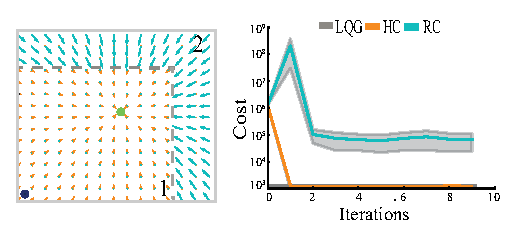
\includegraphics{f_figs/p_mass.eps}
\caption{
    \footnotesize
Left: A 2D workspace where a point mass robot is taught to go to the green circle starting from the blue circle. The world is divided into to two regions with different dynamics. The supervisor is computed via infinite horizon LQG for each region, which results in two different linear matrices in region 1 and 2. Right: RC fails to converges because it is attempting to learn a policy across the two regions, whereas HC remains in region 1 and converges to the supervisor performance. }
\vspace*{-1pt}
\label{fig:p_mass}
\end{figure}

\subsection{Real-World Problem}
Thus far we have seen that the advantage of RC over HC decreases as expressiveness increases on random toy problems. Next, we perform a pilot user study o n a real robot to test performance in practices.
Participants teach the robot to perform a singulation task (i.e. separate an object from its neighbors), illustrated in Fig. \ref{fig:izzy_sing}. A successful singulation means at least one object has its center located 10 cm or more from all other object centers. 

Our hypothesis is that HC will outperform RC in practices when using an expressive learner, for two reasons: 1) RC sampling will force the robot to try and learn more complex behavior. 2) Participants will struggle with providing retroactive feedback. 

The robot has a two-dimensional control space, $\mathcal{U}$, of base rotation and arm extension. The state space of the environment, $\mathcal{X}$, is captured by an overhead Logitech C270 camera, which is positioned to capture the workspace that contains all cluttered objects and the robot arm.  The objects are red extruded polygons. We consider objects made of Medium Density Fiberboard with an average 4" diameter and 3" in height.  We use the current image of the environment as the state representation, which captures positional information. The policy is a deep neural network with the architecture from~\cite{laskeyrobot}. The network is trained using TensorFlow~\cite{tensorflow2015-whitepaper} on a Telsa K40 GPU. 

\begin{figure}
\centering

\includegraphics{f_figs/singulation.eps}
\caption{
    \footnotesize
Left: An example initial state the robot observes. The initial state can vary the relative position of the objects and pose of the pile. Right: A human is asked to singulate the object, which is to have the robot learn to push one object away from its neighbors. A successful singulation means at least one object has its center located 10 cm or more from all other object centers.   }

\label{fig:izzy_sing}
\end{figure}


\begin{figure}
\centering
\includegraphics{f_figs/labeling.eps}
\caption{
    \footnotesize
Two ways to provide feedback to the robot. a)In HC sampling, the human teleoperates the robot and performs the desired task. For the singulation task, the human supervisor used an Xbox Controller. b) In RC sampling, the human observes a video of the robot's policy executing and applies retroactive feedback for what the robot should have done. In the image shown, the person is telling the robot to go backward towards the cluster.  }

\label{fig:labeling}
\end{figure}

The robot is moved via positional control implemented with PID. Similar to \cite{laskeyshiv}, the control space $\mathcal{U}$ consists of bounded changes in rotation and translation. The control signals for each degree of freedom are continuous values with the following ranges: base rotation, $[-1.5^\circ,1.5^\circ]$, arm extension $[-1cm,1cm]$.

\jmnote{Tense change here, fix at some point}
During training and testing the initial state distribution $p(\bx_0)$ consisted of sampling the 2D pose of the object cluster from a multivariate Gaussian \mlnote{get numbers}.The relative position of the 4 objects is sampled from a uniform distribution. To help a human operator place objects in the correct pose, we used a virtual overall over the webcam.   

Each participant trains the robot in both HC and RC sampling (a within-subjects design). In HC, we asked participants to provide 60 demonstrations to the robot using an Xbox Controller, as shown in Fig. \ref{fig:labeling}a. In RC, participants provided 20 initial demonstrations via the Xbox Controller, and then provided retroactive feedback for $K=2$ iterations of 20 demonstrations each.

Retroactive feedback is provided through a labeling interface similar to Laskey et al. \cite{laskeyrobot}, illustrated in Fig \ref{fig:labeling}b. In this interface, we showed a video at half speed of the robot's rollout to the participant. They then use a mouse to provide feedback in the form of translation and rotation. We provide a virtual overlay so that they can see the magnitude of their given control. 

We selected 10 UC Berkeley students as human subjects. The subjects were familiar with robotics, but not the learning algorithms behind the techniques. They first watched a trained robot perform the task successfully.  They then practiced providing feedback through RC sampling for 5 demonstrations and HC for 5 demonstrations. Next, each subject performed the first 20 demonstrations via HC sampling. Then they performed 40 HC demonstrations and 40 RC demonstrations in a counter-balanced order.  The experiment took 2 hours per person on average. 

\begin{figure}
\centering
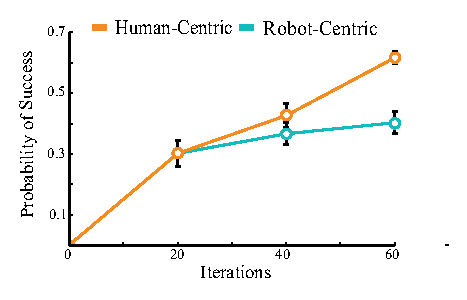
\includegraphics{f_figs/izzy_reward.eps}
\caption{
    \footnotesize
Average success at the singulation task over the 10 human subjects as a function of number of demonstrations. Each policy is evaluated 30 times on the a held out set of test configurations. The first 20 rollouts are from the supervisor rolling out there policy and the next 40 are collected via retro-active feedback for RC and tele-operated demonstrations for HC. HC LfD shows a 20$\%$ improvement in success at the end. }

\label{fig:izzy_rw}
\end{figure}

In Fig. \ref{fig:izzy_rw} , we show the average performance of the policies trained with RC and HC LfD. Each policy is evaluated on a holdout set of 30 initial states sampled from the same distribution as training.
The policies learned with RC have approximately $40\%$ probability of success versus $60\%$ for HC, and the result is statistically significant\mlnote{send data to Anca}.
This suggests that HC may outperform RC when supervision is provided by actual human demonstrations.

\subsection{Understanding RC Performance in Practice}
To better understand why RC performed worse than HC, we looked for the two causes in our hypothesis: policy complexity, and human supervision difficulty.

\noindent\textbf{Policy Complexity: }We first analyzed the complexity of behaviors collected with RC sampling. In Fig. \ref{fig:teaser}c, we show trajectories collected on a single initial state during the study. As illustrated, HC sampling is concentrated around a path needed to singulate the bottom right object. However, RC sampling places the robot in a wide variety of states, some of which would require the robot learning how to move backward or rapidly change direction to recover. 

To better analyze this, we examined the surrogate loss on a test set of 10 randomly selected trajectories from each supervisor's dataset.  As shown in Table 1, we observed the average test error over the policies trained with 60 demonstrations in both degrees of freedom (i.e. translation and rotation) is significantly higher.
This indicates that the RC policies had a harder time generalizing to unseen labels in their aggregate dataset on average, which may be due to the complexity of the corrective actions.

\begin{table}[t]
\centering
\begin{tabular}{ R{1.75cm}||R{2.5cm}| R{2.5cm}}
 %\hline
 %\multicolumn{4}{|c|}{Sensitivity Analysis for Convergence to Best Grasp for Thompson sampling} \\
 %\hline 
 & \multicolumn{2}{c}{Surrogate Loss on Test Set} \\
 \hline
\specialcell{\bf Algorithm\\ \bf Type} & \specialcell{\bf Translation \bf (mm)} & \specialcell{\bf Rotation \\ \bf (rad)} \\
 \hline
HC LfD & $2.1\pm 0.2$ & $0.009 \pm 0.001$ \\
RC LfD & $3.4 \pm 1.0$    & $0.014 \pm 0.003$ \\
 %\hline
\end{tabular}
   \caption { \footnotesize  The average surrogate loss on a held out set of 10 demonstrations from the the total 60 demonstrations collected for each 10 participants. The confidence intervals are standard error on the mean, which suggest that RC LfD obtains a statistically significant higher surrogate loss in both degrees of freedom, forward and rotation. 
   }
		\tablabel{opt-p-comparison}
\vspace*{-10pt}
\end{table}



\begin{figure}
\centering
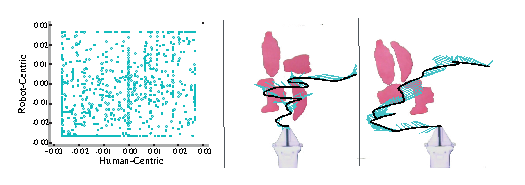
\includegraphics{f_figs/cor_data.eps}
\caption{
    \footnotesize
    Results from the post analysis examining how well retroactive feedback matched teleoperation. The scatter plot shows the normalized angle of the control applied for both HC (teleoperation) and RC (retroactive).  The large dispersion in the graph indicates that the five participants had a difficult time matching their retroactive and teleoperated controls. Two example trajectories are also shown.  The black line indicates the path from teleoperation and the teal line is the direction and scaled magnitude of the feedback given. If they matched perfectly, the teal line would be tangent to the path. 
}

\label{fig:izzy_traj}
\end{figure}


\noindent\textbf{Human Supervision. }We next hypothesized that the participants could have had trouble providing retroactive feedback that is consistent with their true policy. To test this, we asked 5 of the participants to provide 5 demonstrations via teleoperation. Then we asked them to match their controls via the RC labeling interface. 

We measured the correlation between the controls applied via retroactive feedback and teleoperation. When calculated over all the participants and trajectories, the Pearson Correlation Coefficient in rotation and translation was 0.60 and 0.22, respectively. A smaller correlation coefficient suggests that it is harder for people to match their control in teleoperation. 

In Fig. \ref{fig:izzy_traj} we plot the control angle from HC sampling versus the control angle from RC sampling, showing that the two are not correlated. We also show two trajectories that a participant teleoperated with their retroactive labels overlayed, both of which suggest disagreement between the teleoperated and retroactive controls. Overall, our analysis suggests that RC sampling can lose the intent of the human supervisor. 

\section{Theoretical Analysis}
To better understand the empirical results from above, we contribute new theoretical analysis on RC and HC LfD. In this section, we first show the existence of environments where HC converges to the supervisor but RC does not. Then we present a new analysis of the accumulation of error for \ns. 


\section{Theoretical Analysis} 

\subsection{Algorithm Consistency}\label{sec:consistent}
In this section we work towards a fuller understanding of the tradeoffs between HC and RC. 
One of the motivations for the use of the RC LfD algorithm is that the feedback from the supervisor is being provided for the trajectory that is the result of executing the latest learned policy.
That is, instead of the supervisor repeatedly demonstrating the task over and over to the robot without any corrective feedback to the robot's learned policy (as is done in HC LfD), at each time in RC LfD the robot attempts the task with what knowledge it has gained about the task so far and the supervisor provides feedback on this attempt. 
The RC approach is particularly appealing when the robot's policy is incapable of matching the supervisor's demonstrations exactly.  
This intuition along with a theoretical analysis of Ross et al. ~\cite{ross2010reduction} has led to use of the RC approach~\cite{zhang2016query,he2012imitation,ross2013learning}.

The analysis of RC LfD in \cite{ross2010reduction} is performed in the context of the regret framework of online learning. 
In online learning, at each iteration $k \in \{1,\dots,n\}$ the algorithm chooses an action $\theta_k \in \Theta$ (e.g. a policy to roll out), and observes some loss $f_k(\theta_k)$. 
Online learning is analyzed in the context of a regret guarantee: a function of $n$ (e.g. $\sqrt{n}$) that upper bounds the cumulative loss incurred by the algorithm relative to taking just the best single action in $\Theta$:

\begin{align*}
\sup_{\theta \in \Theta} \sum_{k=1}^n f_k(\theta_k) - f_k(\theta).
\end{align*}

For instance, in the context of linear binary classification $\theta_k$ could be a linear predictor and $f_k(\theta)= 1\{ y_k \neq \text{sign}(x_k^T\theta) \}$ where $(x_k,y_k)$ example-label pairs from some streaming dataset. 
In this classification example, comparing to the best single $\theta \in \Theta$ that could have been played for all loss functions $f_1,f_2,\dots,f_n$ makes sense because the $f_k$ functions are presumably uncoupled from the actions taken $\{\theta_j\}_{j \leq k}$: $\inf_{\theta \in \Theta} \sum_{k=1}^n f_k(\theta)$ is just the familiar empirical risk minimizer. 
However, in the context of robotics and specifically in the case of RC LfD, taking an action $\theta_k$ at iteration $k$ is rolling out a policy dictated by $\theta_k$ which induces a series of states $\bx_{k,1},\dots,\bx_{k,T}$ and the loss is evaluated with respect to {\em these} states.  

Under these circumstances, a regret bound of this form is potentially not indicative of the absolute performance on the task.
For instance, consider a car-racing game where the car has constant speed and the controller can only decide to go left and right. Suppose the game encounters a ``v'' in the road where one path is a well-paved road and the other path is a muddy dirt road with obstacles. Suppose the algorithm played a series of policies $\theta_1,\dots,\theta_k$ where each policy dictated that the car takes the dirt road. The instant that the algorithm made the wrong decision at the ``v'' would be penalized by the supervisor, but at every instance once the car is on the dirt path the car may be acting optimally, making the best of a bad situation (or worse, the supervisor focuses all its energy on teaching the car how to drive on a muddy dirt road). In this situation, obviously the policy never should have taken the car down the dirt path and should have stayed on the paved road resulting in a better time, but because the car acted optimally once it was on the dirt path, this dirt-road sequence of policies would have very low regret!
Intuitively, RC LfD is performing a greedy strategy for optimization and has the potential to get stuck in local minima because the states induced by the played policy may not be informative to identifying global solutions.

The next theorem formalizes this intuition.


\begin{theorem}
For a given environment (state space, action space, dynamics mapping state-action pairs to states, and a loss function) and policy class $\Theta$,
let $\theta_{HC}^N$ be the policy learned from $N$ supervisor demonstrations,
and let $\theta_{RC}^N$ be the policy learned by the $RC$ procedure described in Section~\ref{} that is initialized with $m$ supervisor demonstrations.  
Then there exists an environment and policy class $\Theta$ such that 
\begin{itemize}
\item $\theta^*$ is the unique minimizer of $E_{p(\tau \mid \theta)}[ J( \theta ) ]$,
\item $\lim_{N \rightarrow \infty} \theta_{HC}^N = \theta^*$ with probability $1$,
\item $\lim_{N \rightarrow \infty} \theta_{RC}^N \neq \theta^*$ with probability at least $c e^{-m}$
\end{itemize}
for some universal constant $c$.
In other words, even with infinite data RC may converge to a suboptimal policy while HC converges to the best policy in the class that uniquely achieves the lowest loss.
\end{theorem}

\begin{figure}
\centering
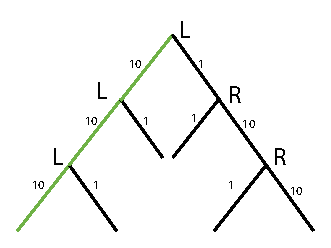
\includegraphics{f_figs/counter_exmp.eps}
\caption{
    \footnotesize
A Directed Acyclic Graph, where a robot is being taught by a supervisor to descend down and achieve maximum cumulative reward, which is shown via the numbers on each branch. Each node has the action the supervisor would select, either left or right, $\lbrace L, R \rbrace$. The HC method converges to the Orange path, which is optimal. While the RC method converges to the Teal path, because it tries to learn on examples from that side of the tree.}
\vspace*{-20pt}
\label{fig:c_ex}
\end{figure}


\begin{proof}
Let $\{ \{ (\bx_{k,t},\bu_{k,t} \}_{t=0}^3 \}_{k=1}^N$ denote $N$ trajectories.
Consider an environment with a deterministic initial state at the root of the DAG of Figure~\ref{fig:c_ex} so that $p(\bx_{k,0} = \texttt{root}) = 1$ for all $k$. 
The space of policies are constant functions $\Theta = \{L,R\}$ where if $\theta=L$ then regardless of the state, the control input $\bu_{k,t}$ will be to take the left child (and analogously for $\theta=R$ taking the right child).
For any state in the DAG with children, let $\phi(\bx_{k,t},\theta)$ denote the left child of $\bx_{k,t}$ if $\theta=L$ and the right child otherwise. 
The dynamics are described as follows: for some $\mu \in (0,1/4]$ to be defined later, if $\theta=L$ and $\bx_{k,t}=\texttt{root}$ then $p(\bx_{k,1}=\phi(\bx_{k,0},R))=\mu$ and $p(\bx_{k,1}=\phi(\bx_{k,0},L))=1-\mu$, but if $\theta=R$ then the right child is chosen with probability $1$. If $\bx_{k,t} \neq \texttt{root}$ then $\bx_{k,t+1} = \phi(\bx_{k,t},\theta)$.

Assume that the supervisor $\pi^*: \mathcal{X} \rightarrow \{L,R\}$ acts greedily according to the given rewards given in the DAG so that $\pi^*(\bx_{k,t})=L$ if the reward of the left child exceeds the right child and $\pi^*(\bx_{k,t})=R$ otherwise.
Finally, define the state loss function $\ell(\cdot,\cdot)$ as the $0/1$ loss so that after $N$ trajectories, the loss is given as $J_N(\theta)=\sum_{k=1}^N \sum_{t=0}^2 \mathbf{1}\{ \pi^*(\bx_{k,t}) \neq \theta \}$ for all $\theta \in \{L,R\}$. Note that $\widehat{\theta}_N = \arg\min_{\theta \in \{L,R\}} J_N(\theta)$ is equivalent to looking at all actions by the supervisor over the states and taking the majority vote of $L$ versus $R$ (i.e. the states in which these actions are taken has no impact on the minimizer). Note that we have not yet specified how the states $\bx_{k,t}$ were generated. 

We can compute the true loss when the trajectories are generated by $\theta \in \{L,R\}$. Let the empirical distribution of observed states under a fixed action $\theta \in \{L,R\}$ be given by $p(\tau \mid \theta)$, then
\begin{align*}
 E_{p(\tau \mid \theta=L) } J(\theta=L) &= p( \bx_{k,1} = \phi(\bx_{k,0},L) ) \cdot 0 + p( \bx_{k,1} = \phi(\bx_{k,0},R) ) \cdot 2  = 2 \mu\\
   E_{p(\tau \mid \theta=R) } J(\theta=R) &= 1
\end{align*}
which implies that $\theta_* = L$ and performs strictly better than $R$ whenever $\mu < 1/2$.

It follows by the stochastic dynamics that the demonstrated action sequence by the supervisor equals $\{L,R,R\}$ with probability $\mu$ and $\{L,L,L\}$ with probability $1-\mu$.
After $m$ supervisor sequences, the expected number of $L$ actions is equal to $\mu+3(1-\mu)=3-2\mu$ while the expected number of $R$ actions is equal to just $2\mu$.
By the law of large numbers, if only supervisor sequences are given then $\arg\min_{\theta \in \{L,R\}} J_m(\theta) \rightarrow L = \theta^*$ as $m \rightarrow \infty$ since $3-2\mu>2\mu$ for all $\mu<1/2$. 
In other words, $\theta_{HC}^N \rightarrow \theta^*$ as $N \rightarrow \infty$.

We now turn our attention to $RC$'s policy.
Note that if after $m$ supervisor action sequences we have that the number of observed $R$'s exceeds the number of observed $L$'s, then $RC$ policy will define $\theta_{RC}^m = R$. 
It is easy to see that a policy rolled out with $\theta=R$ will receive the supervisor's action sequence $\{L,R,R\}$ and thus $R$ will remain the majority vote and consequently $\theta_{RC}^N=R$ for all $N \geq m$.
What remains is to lower bound the probability that given $m$ supervisor demonstrations that $\theta_{RC}^m = R$. 

For $k=1,\dots,m$ let $Z_k \in \{0,1\}$ be independent Bernoulli($\mu$) random variables where $Z_k=1$ represents observing the supervisor sequence $\{L,R,R\}$ and $Z_k=0$ represents observing $\{L,L,L\}$.
Given $m$ supervisor sequences, note that the event $\arg\min_{\theta \in \{L,R\}} J_m(\theta) = R$ occurs if $\frac{1}{m}\sum_{k=1}^m Z_k > 3/4$. 
Noting that $\sum_{k=1}^m Z_k$ is a binomial($m$,$\mu$) random variable, the probability of this event is equal to 
\begin{align*}
\sum_{k=\lfloor 3m/4 \rfloor+1}^m \binom{m}{k} \mu^k (1-\mu)^{m-k} \geq \Phi\left( \frac{\lfloor 3m/4 \rfloor+1 - \mu m}{ \sqrt{m \mu(1-\mu)}} \right) 
\end{align*} 
where we have used Slud's inequality \cite{slud1977} to lower bound a binomial tail by a Gaussian tail. 
Setting $\mu=1/4$ we can further lower bound this probability by $\Phi\left( \frac{m + 2}{ \sqrt{3m/4}} \right) \geq c e^{-m}$ for some universal constant $c$.
Consequently, with probability at least $c e^{-m}$ we have that $\lim_{N \rightarrow \infty} \theta_{RC}^N = R \neq \theta^*$ which implies that the expected loss of $\lim_{N \rightarrow \infty} \theta_{RC}^N$ must exceed the expected loss of $\theta_*=L$.
\end{proof}





\
\subsection{Bound on Error for HC Lfd}
In the HC LfD setting a robot is trained on the states visited by the supervisor. However, at run time the robot may encounter a different distribution of states due to not perfectly matching the supervisor's policy. Ross et al. showed that given a time horizon, $T$, the worst case error scales quadratically (i.e. $O(T^2E_{p(\bx|\theta^*)} l(\theta^N)$) when executing the robot's policy~\cite{ross2010efficient}. Note according to the notation of Ross et al., $TE_{p(\bx|\theta^*)} l(\theta^N) = E_{p(\tau|\theta^*)} J(\theta^N, \tau)$. We present a new analysis for a class of stochastic policies and  defined below that shows a rate of $O(T\sqrt{TE_{p(\bx|\theta^*)} l(\theta^N)})$ (See Supplement Material). 


\section{Discussion}
 Our results suggest that the RC methods can have an overhead cost when being implemented on a real system. The cost can occur from either the robot observing complex recovery actions or retroactive feedback losing the intention of human supervisors. Fortunately, results suggest HC can achieve similar performance as the robot's policy becomes more expressive. 

We note though there are limitations to using these very expressive models. The non-convex optimization required to train deep neural networks can be prone to a local minimum, which means learning error may not always be minimized. Furthermore, expressive models can be more susceptible to noise from humans than shallower function classes, which could require more data. 

In future work, we will examine how to instruct human supervisors to provide better demonstrations, which may make them less noisy. Furthermore, we are interested in knowing exactly how much data is needed to achieve high reliability on tasks with significant variance in the initial state. A better theoretical understanding of the sample complexity associated with HC LfD can help answer this question. 




\bibliographystyle{IEEEtranS}
\bibliography{references}


\appendix
\mlnote{This will go into a supplement material. Kevin raises a good point that we shouldn't promote bounds with random variables in them. Theorem 6.1 shows exactly what that is a bad idea. We will save understanding how to get a data-dependent rate on this for future work}

 Define the surrogate loss as the squared euclidean norm, or $l(\pi_{\theta}(\bx),\pi_{\theta^*}(\bx)) = ||\pi_{\theta}(\bx_{i,t}) - \pi_{\theta^*}(\bx_{i,t})||_2$.We assume that the controls are be bounded and thus can be normalized such that the $l \in [0,1]$.  We are interested in the situation where the supervisor and robot policy are stochastic with a Normal Distribution (i.e. $p(\bu|\pi_{\theta}(\bx)) = \mathcal{N}(\pi_\theta(\bx),\sigma I)$. The interest in stochastic policies instead of deterministic is two-fold: 1) human supervisor can be noisy in nature and 2) due to noise in robot execution, such as cable coupling, the intended and actual control may differ in a stochastic way~\cite{mahler2014learning}. \mlnote{need to clarify what the generalization is} We show a generalization of this bound to any distribution in the exponential family in the supplement material.  Note Ross et al.~\cite{ross2010reduction} used a deterministic policy in their analysis, which may prohibit a direct comparison of rates. To be concise we refer to $J(\theta, \tau)$ as $J(\theta)$, dropping the reference to a trajectory.

\begin{theorem}
Given a policy $\pi_{\theta^N}$, the following is true 
$$E_{p(\tau|\theta^n)} J(\theta^N) \leq T\sqrt{\frac{1}{4\sigma}E_{p(\tau|\theta^*)} J(\theta^N)}+E_{p(\tau|\theta^*)} J(\theta^N)$$
\end{theorem}
\begin{proof}
For convenience we will write $E_{p(\tau|\theta)} = E_{\theta}$ and $l(\theta,\bx) = l(\theta)$. The proof follows by first deriving an upper bound on the worst case difference between the two quantities $E_{\theta^N} J(\theta^N) - E_{\theta^*} J(\theta^N) $. Then we leverage the intuition that if one is minimizing $E_{\theta^*} J(\theta^N) $, they are also decreasing the distance between the robot and supervisor's distributions. 

\begin{align}
&E_{\theta^N} J(\theta^N) - E_{\theta^*} J(\theta^N) \\
&= T(\frac{1}{T}E_{\theta^N} J(\theta^N) -\frac{1}{T}E_{\theta^*} J(\theta^N)\\
&\leq  T| | p(\tau|\theta^N) - p(\tau|\theta^*)||_{TV}\\
&\leq T\sqrt{\frac{1}{2} D_{KL}(p(\tau|\theta^*),p(\tau|\theta^N))}
\end{align}

 Line 6 leverages the fact that the worst case loss is bounded by $1$ and the definition of Total Variational distance. Line 7 uses Pinsker's inequality~\cite{verdu2014total}.


\begin{align}
&= T\sqrt{\frac{1}{2} E_{p(\theta^*)} \mbox{log} \frac{p(\tau|\theta^*)}{p(\tau|\theta^N)}}\\
&= T\sqrt{\frac{1}{2} E_{p(\theta^*)} \sum^T_{t=1}\mbox{log} \frac{p(\bu_t|\bx_t,\theta^*)}{p(\bu_t|\bx_t,\theta^N)}}\\
&= T\sqrt{\frac{1}{4\sigma} E_{p(\theta^*)} \sum^T_{t=1} ||\bu_t- \pi_{\theta^N}(\bx_t)||_2^2 - ||\bu_t- \pi_{\theta^*}(\bx_t)||_2^2}\\
&\leq T\sqrt{\frac{1}{4\sigma} E_{p(\theta^*)} \sum^T_{t=1}  ||\pi_{\theta^*}(\bx_t) - \pi_{\theta^N}(\bx_t)||_2^2}\\
&= T\sqrt{\frac{1}{4\sigma} E_{p(\theta^*)} J(\theta^N)}\\
&= T\sqrt{T \frac{1}{4\sigma} E_{p(\bx|\theta^*)} l(\theta^N)}
\end{align}

Line 8,9 and 10 apply the definition of the KL-divergence, the markov chain and the normal distribution over $p(\bu_t|\bx_t,\theta)$. Line 11 applies the triangle inequality to upperbound by the defined surrogate loss. Line 12 applies the assumed definition of $J(\theta)$. Line 13 uses the notation of Ross et al.. 

The intuition behind these steps is that difference between  the two distribution can be controlled via the surrogate loss on the expected supervisor. Thus, illustrating the closer the robot's policy matches the supervisor's policy on the supervisor's distribution, the smaller the total variational difference between the resulting two distributions will be. 
\end{proof}
  
The above analysis demonstrates how the constant $T$ affects the bound in error. However, it is important to note that this is not the only variable that plays a role in performance. The size of the function class and number of demonstrations needed are are also important in determining how large $E_{p(\bx|\theta^*)} l(\theta^N)$ is. 

Understanding how much data is needed to learn a function, is a well studied problem known as sample complexity analysis~\cite{anthony2009neural,bartlett2002rademacher,kakade2009complexity}. In this literature they use different metrics to describe the complexity of a function class and show rates on which a given function class would converge to the best in the set. We refer the reader to \cite{vapnik2013nature}, for a review of such topics. 



\end{document}
Contact GitHub API Training Shop Blog About
© 2016 GitHub, Inc. Terms Privacy Security Status Help
